% ------------------------------------------------------------------------------
% TYPO3 Version 9.4 - What's New (Dutch Version)
%
% @license	Creative Commons BY-NC-SA 3.0
% @link		https://typo3.org/help/documentation/whats-new/
% @language	Dutch
% ------------------------------------------------------------------------------


\section{Inleiding}
\begin{frame}[fragile]
	\frametitle{Inleiding}

	\begin{center}\huge{Inleiding}\end{center}
	\begin{center}\huge{\color{typo3darkgrey}\textbf{De feiten}}\end{center}

\end{frame}

% ------------------------------------------------------------------------------
% TYPO3 Version 9.4 - The Facts

\begin{frame}[fragile]
	\frametitle{Inleiding}
	\framesubtitle{TYPO3 Versie 9.4 - De feiten}

	\begin{itemize}
		\item Publicatiedatum: 04 september 2018
		\item Publicatietype: Sprint Release
	\end{itemize}

	\begin{figure}
		
\includegraphics[width=0.95\linewidth]{Introduction/typo3-v94-banner.jpg}
	\end{figure}

\end{frame}

% ------------------------------------------------------------------------------
% System Requirements

\begin{frame}[fragile]
	\frametitle{Inleiding}
	\framesubtitle{Systeemeisen}

	\begin{itemize}
		\item PHP versie 7.2 of hoger
		\item PHP instellingen:

			\begin{itemize}
				\item \texttt{memory\_limit} >= 256M
				\item \texttt{max\_execution\_time} >= 240s
				\item \texttt{max\_input\_vars} >= 1500
				\item compilatieoptie \texttt{-}\texttt{-disable-ipv6} moet \underline{niet} worden gebruikt
			\end{itemize}

		\item De meeste databaseservers die worden ondersteund door \textbf{Doctrine DBAL} werken ook met TYPO3.
			De geteste database systemen zijn:
	\end{itemize}

	\begin{figure}
		
\includegraphics[width=0.80\linewidth]{Introduction/logo-databases.png}
	\end{figure}

\end{frame}

% ------------------------------------------------------------------------------
% Development, Release and Maintenance Timeline

\begin{frame}[fragile]
	\frametitle{Inleiding}
	\framesubtitle{Ontwikkeling-, versie- en onderhouds-tijdlijn}

	\textbf{TYPO3 v9}

	\begin{figure}
		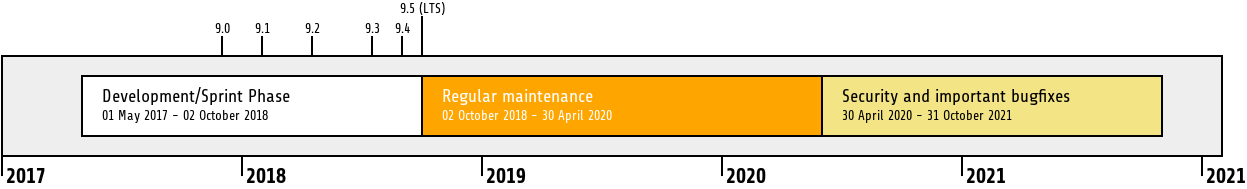
\includegraphics[width=1\linewidth]{Introduction/typo3-v9-lifecycle.png}
	\end{figure}

	\textbf{Verlengde ondersteuning}\newline
	\smaller
		De \href{https://typo3.com}{TYPO3 GmbH} biedt nog 2 jaar extra ondersteuning aan
		voor TYPO3 v9 LTS, zelfs na 31 oktober 2021.
	\normalsize

%	\url{https://typo3.com/our-services/extended-support/}

\end{frame}

% ------------------------------------------------------------------------------
% TYPO3 v9 Roadmap

\begin{frame}[fragile]
	\frametitle{Inleiding}
	\framesubtitle{TYPO3 v9 Roadmap}

	Verwachte verschijningsdata en de focus van de versie:

	\begin{itemize}

		\item v9.0 \tabto{1.1cm}12/Dec/2017\tabto{3.4cm}Install Tool en paginaboom herschreven,\newline
			\tabto{3.4cm}Vertalen pagina's verbeterd
		\item v9.1 \tabto{1.1cm}30/Jan/2018\tabto{3.4cm}Redirect afhandeling
		\item v9.2 \tabto{1.1cm}10/Apr/2018\tabto{3.4cm}Site configuratie
        \item v9.3 \tabto{1.1cm}12/Jun/2018\tabto{3.4cm}SEO en URL Routing voorbereiding
		\item
			\begingroup
				\color{typo3orange}
                    v9.4 \tabto{1.1cm}04/Sep/2018\tabto{3.4cm}URL Routing voor pagina's
			\endgroup
		\item v9.5 \tabto{1.1cm}02/Oct/2018\tabto{3.4cm}LTS versie

	\end{itemize}

	\smaller
		\url{https://typo3.org/article/typo3-v9-roadmap/}\newline
		\url{https://typo3.org/cms/roadmap/}
	\normalsize

\end{frame}

% ------------------------------------------------------------------------------
% Installation

\begin{frame}[fragile]
	\frametitle{Inleiding}
	\framesubtitle{Installatie}

	\begin{itemize}
		\item Officiële \textit{klassieke} installatieprocedure op Linux/Mac OS X\newline
			(DocumentRoot bijvoorbeeld \texttt{/var/www/site/htdocs}):
		\begin{lstlisting}
$ cd /var/www/site
$ wget --content-disposition get.typo3.org/9.4
$ tar xzf typo3_src-9.4.0.tar.gz
$ cd htdocs
$ ln -s ../typo3_src-9.4.0 typo3_src
$ ln -s typo3_src/index.php
$ ln -s typo3_src/typo3
$ touch FIRST_INSTALL
		\end{lstlisting}

		\item Symbolische koppelingen op Microsoft Windows:

			\begin{itemize}
				\item Gebruik \texttt{junction} op Windows XP/2000
				\item Gebruik \texttt{mklink} op Windows Vista en Windows 7
			\end{itemize}

	\end{itemize}
\end{frame}

% ------------------------------------------------------------------------------
% Installation using composer

\begin{frame}[fragile]
	\frametitle{Installation and Upgrade}
	\framesubtitle{Installatie met \texttt{composer}}

	\begin{itemize}
	\framesubtitle{Installatie met \texttt{composer}}

			\begin{lstlisting}
$ cd /var/www/site/
$ composer create-project typo3/cms-base-distribution CmsBaseDistribution ^9
			\end{lstlisting}

		\item Of anders kan een maatwerk \texttt{composer.json} bestand gemaakt worden en dan:

			\begin{lstlisting}
$ composer install
			\end{lstlisting}

			Een voorbeeld \texttt{composer.json} is te downloaden van:\newline
			\smaller
				\href{https://composer.typo3.org}{https://composer.typo3.org}
			\normalsize

	\end{itemize}
\end{frame}

% ------------------------------------------------------------------------------
